\documentclass[twocolumn]{article}
\usepackage{graphicx}
\usepackage{listings}
\usepackage{booktabs}

\title{Math 308 Exercises 2.8}
\author{Nakul Joshi}

\newcommand{\setsection}[1]{\setcounter{section}{#1}\section{}}
\renewcommand{\thesubsection}{\alph{subsection})}
\newcommand{\includecode}[1]{\lstinputlisting{#1}}
\newcommand{\code}[1]{\lstinline{#1}}

\begin{document}
\lstset{language=R}
\graphicspath{ {./img/} }
\maketitle

\setsection{2}
$
\overline{x}=6.5\\
m=5.5\\
\tilde{x}=2.389726\\
\tilde{m}=2.342779\\
f(\overline{x})\neq \tilde{x}\\
f(m)\neq \tilde{m}
$

\setsection{4}

\subsection{}
\begin{table}[h]
\centering
    \begin{tabular}{ccccc}
    4-8am & 8-Noon & Noon-4pm & 4-8pm & 8-Mid \\
    699   & 1053   & 1048     & 972   & 257   \\
    \end{tabular}
\end{table}
\begin{figure}[h]
\centering
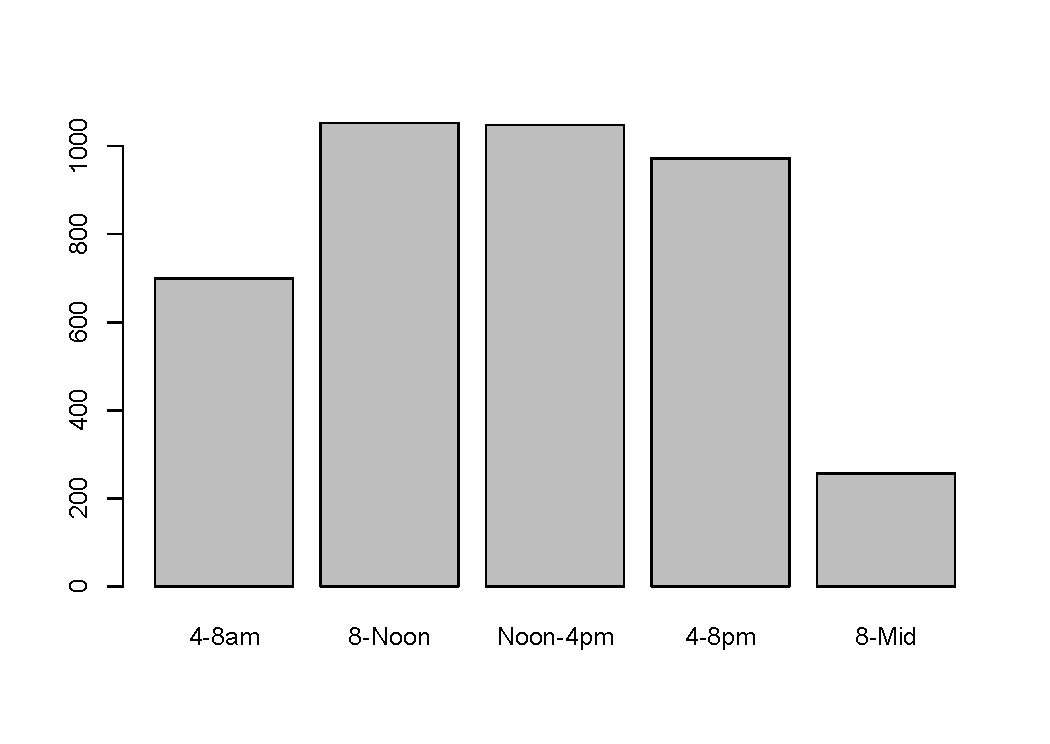
\includegraphics[width=0.4\textwidth]{4a.pdf}
\end{figure}
\newpage

\subsection{}
% Booktabs require to add \usepackage{booktabs} to your document preamble
\begin{table}[h]
\centering
\begin{tabular}{@{}lrrr@{}}
\toprule
  & No  & Yes & Proportion \\ \midrule
Mon & 569 & 61  & 0.09682540 \\
Tue & 535 & 93  & 0.14808917 \\
Wed & 488 & 76  & 0.13475177 \\
Thu & 434 & 132 & 0.23321555 \\
Fri & 493 & 144 & 0.22605965 \\
Sat & 406 & 47  & 0.10375276 \\
Sun & 507 & 44  & 0.07985481\\
\bottomrule
\end{tabular}
\end{table}

\subsection{}
\begin{figure}[h]
\centering
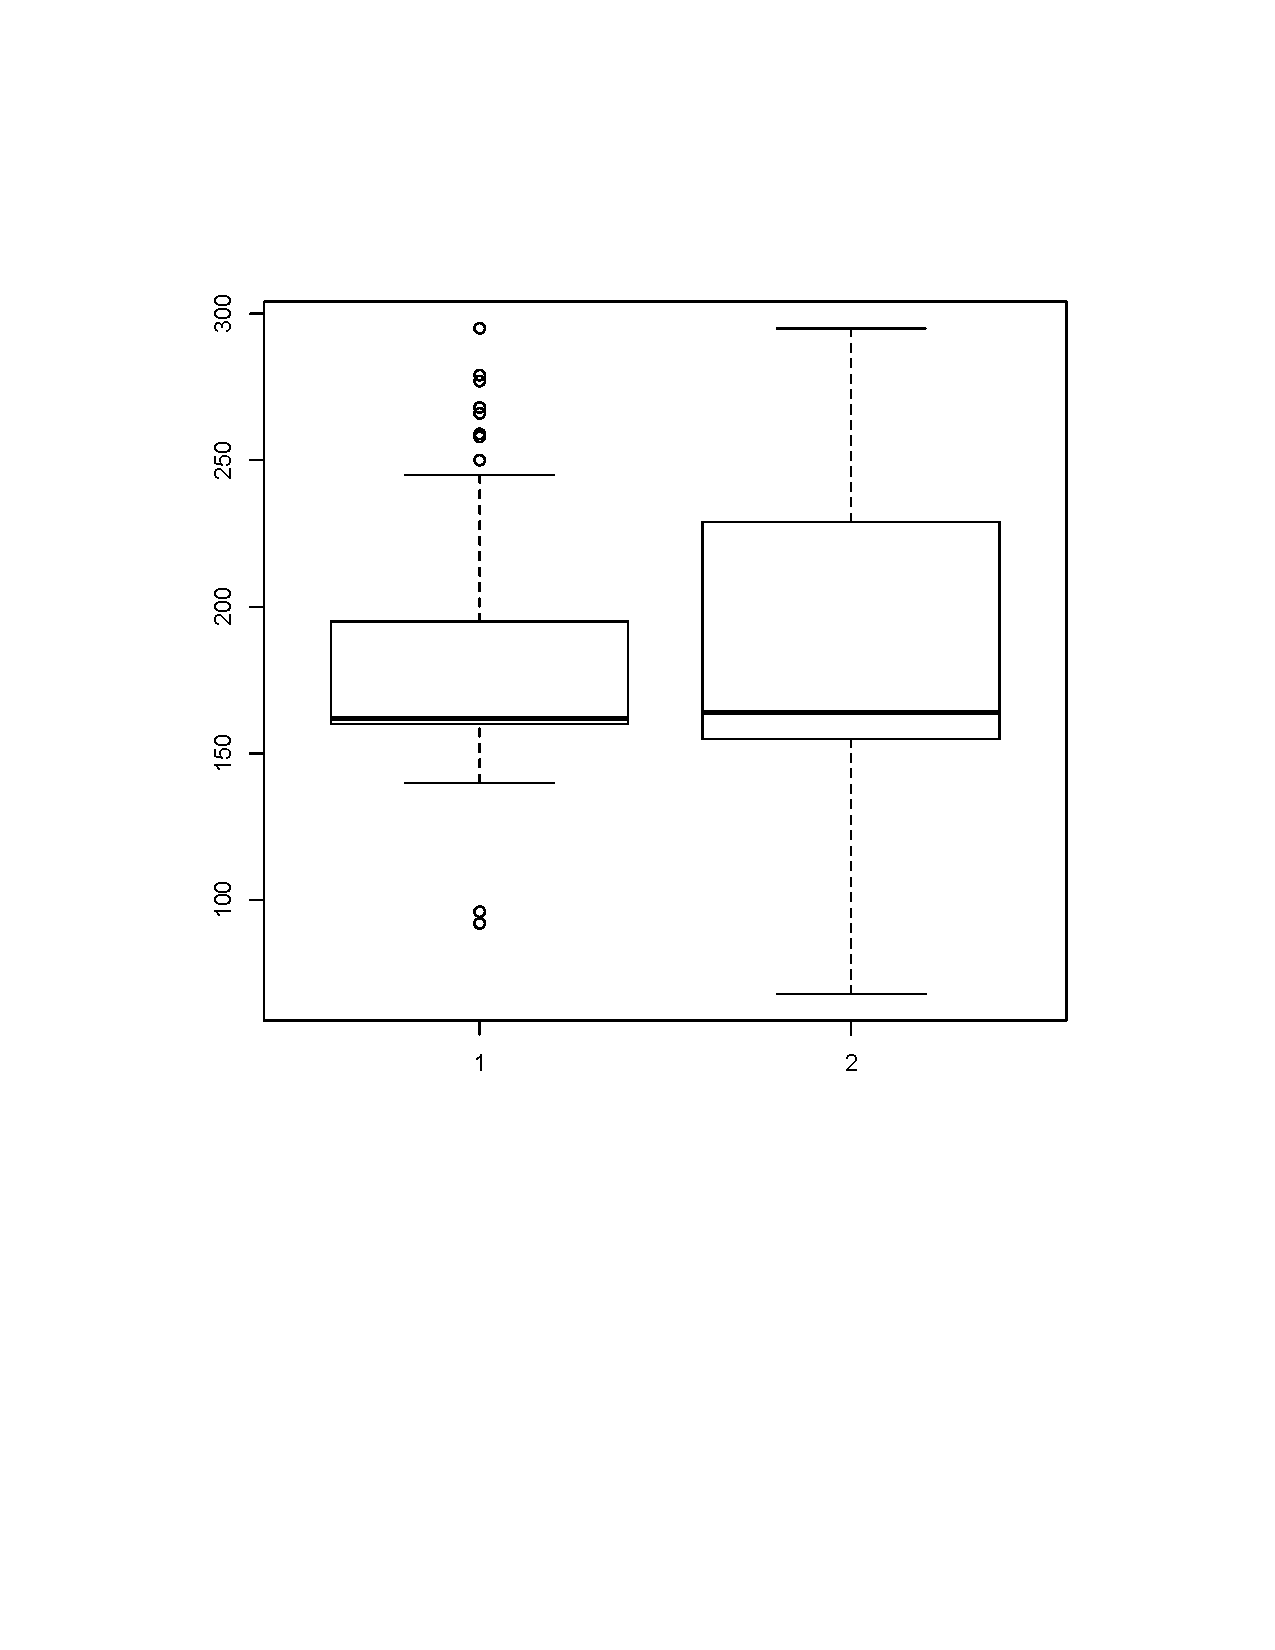
\includegraphics[width=0.4\textwidth]{4c.pdf}
\end{figure}

\subsection{}
There appears to be no relationship.

\setsection{6}

\subsection{}
\begin{table}[h]
\centering
\begin{tabular}{@{}llllll@{}}
\toprule
Min. & 1st Qu. & Median & Mean  & 3rd Qu. & Max.  \\ \midrule
8.30 & 23.20   & 30.10  & 30.93 & 38.17   & 51.50  \\ \bottomrule
\end{tabular}
\end{table}

\subsection{}
\begin{figure}[h]
\centering
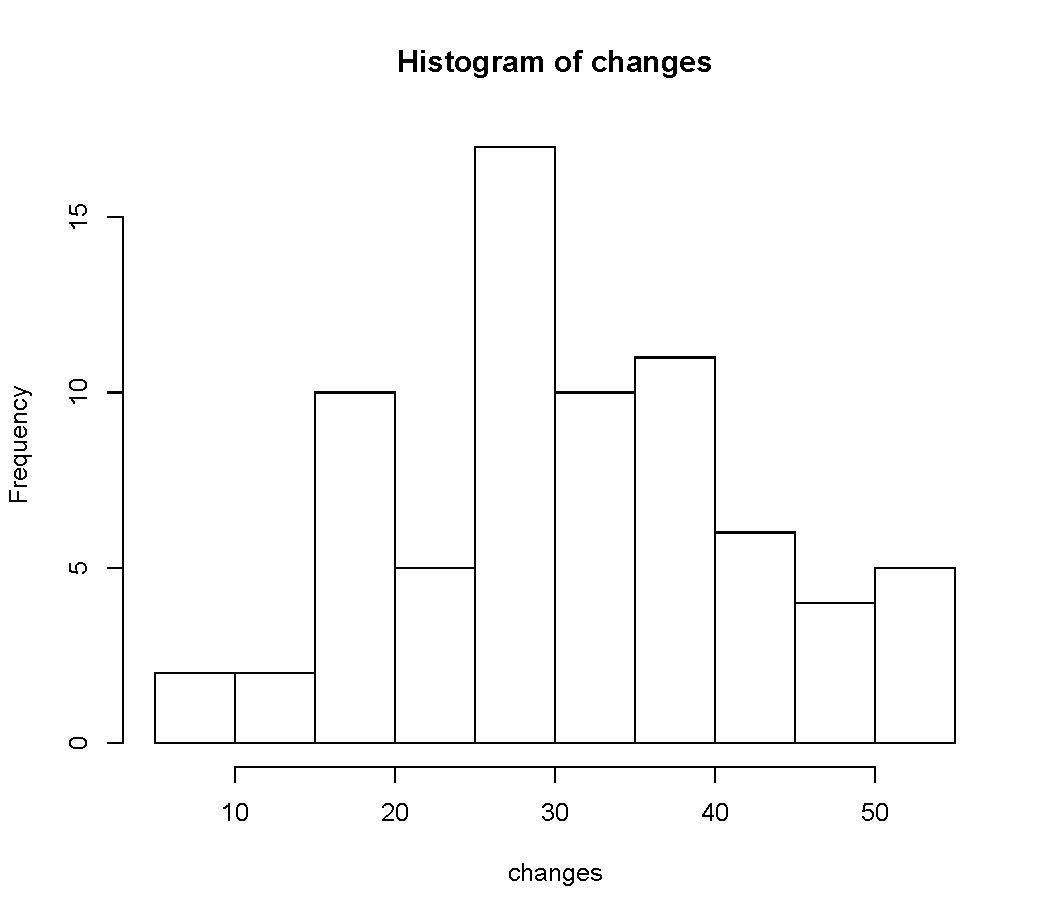
\includegraphics[width=0.4\textwidth]{6b1.pdf}
\end{figure}
\newpage
\begin{figure}[h]
\centering
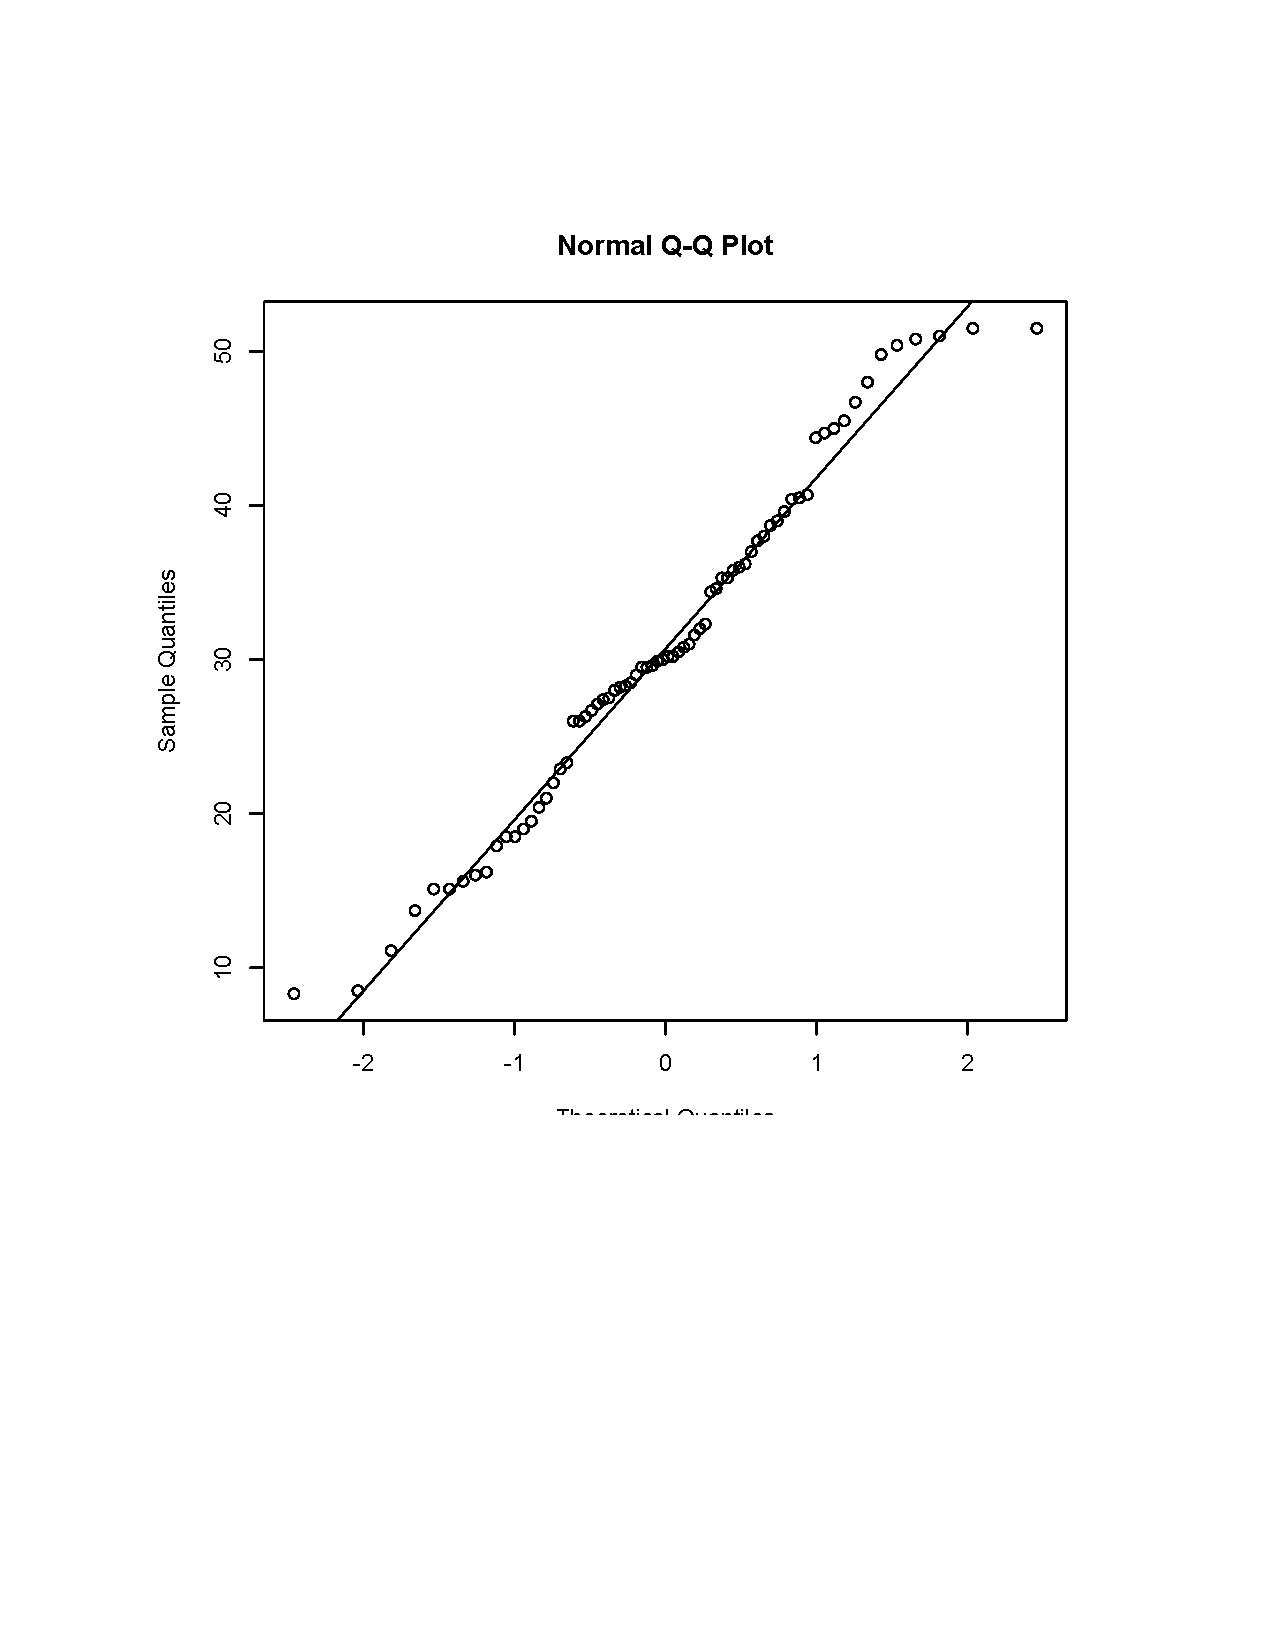
\includegraphics[width=0.4\textwidth]{6b2.pdf}
\end{figure}

The distribution is approximately normal as shown by the close fit between the normal and theoretical quantiles.

\subsection{}
\begin{figure}[h]
\centering
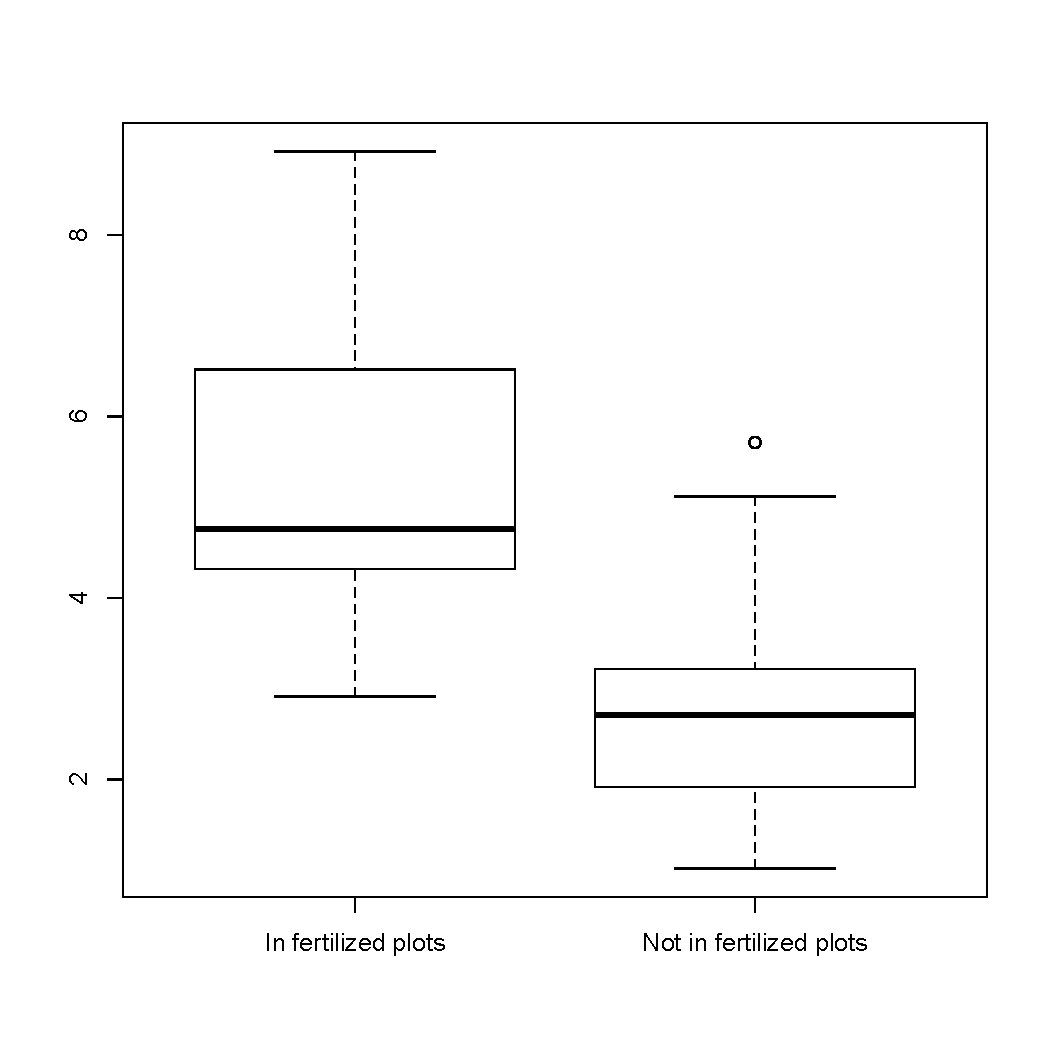
\includegraphics[width=0.4\textwidth]{6c.pdf}
\end{figure}

\newpage

\subsection{}
% Booktabs require to add \usepackage{booktabs} to your document preamble
\begin{table}[h]
\begin{tabular}{@{}llllll@{}}
\toprule
Min.  & 1st Qu. & Median & Mean  & 3rd Qu. & Max.  \\ \midrule
2.912 & 4.318   & 4.762  & 5.274 & 6.518   & 8.919 \\ \bottomrule
\end{tabular}
\caption{Summary of F}
\end{table}
\begin{table}[h]
\begin{tabular}{llllll}
\toprule
Min.  & 1st Qu. & Median & Mean  & 3rd Qu. & Max.  \\ \midrule
1.019 & 1.915   & 2.712  & 2.718 & 3.165   & 5.712 \\ \bottomrule
\end{tabular}
\caption{Summary of NF}
\end{table}

\subsection{}
\begin{figure}[h]
\centering
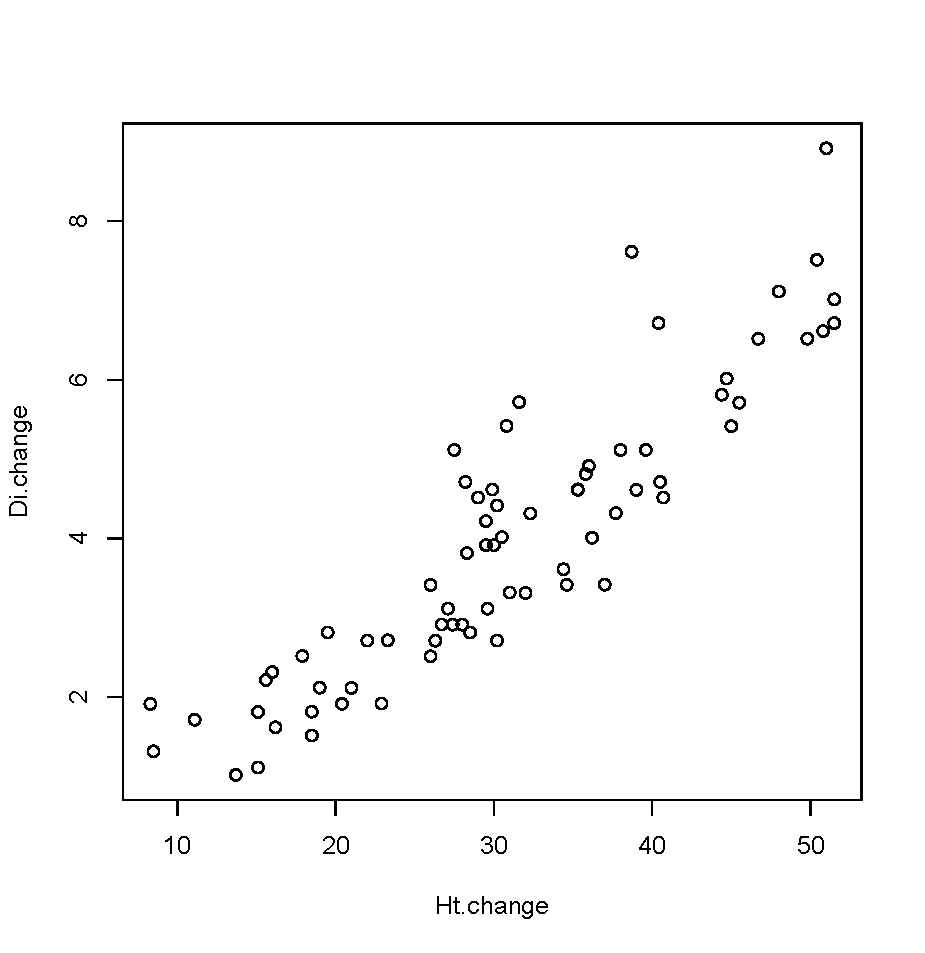
\includegraphics[width=0.4\textwidth]{6e.pdf}
\end{figure}
The diameter changes roughly increase with the height changes.

\end{document}